 \startchapter{Semantic Representations in CNNs}
\label{chapter:Exp}

%Write an introduction here

Convolutional Neural Networks (CNNs), a type of Artificial Neural Network (ANN) loosely inspired by the human visual cortex, has become the state of the art technology in object recognition from images. Over the last five years, the deep learning community has demonstrated that having deeper networks have a direct impact on the performance of these networks~\cite{VGG16,ResNet,Inception-v3}. The trend of going deeper with Convolutional Neural network has lead to the creation of a myriad of black box architectures which works well at the task of object classification. However, there is an apparent lack of understanding on why various CNN architectures perform better than the other.

We propose to study the semantic representations through the hidden layers of various CNN architectures to offer insights on the function and performance of these complicated networks. We propose to use the DS models trained on text corpora that have been widely used to study semantics in the brain to help us explore semantic feature representations through the layers of CNN. This proposed methodology could contribute to better understanding of CNN and potentially pave the way for improved designing and debugging of CNN. To demonstrate an application of our methodology, we conducted experiments to determine where in the hierarchy of the CNN misclassifications emerge. The contributions addressed by this chapter are below (\textit{Contribution B}):

\begin{itemize}
\item{A novel methodology to study semantic representation through hierarchical layers of CNNs.}
\item{The study of hidden representations of images that are misclassified.}
\end{itemize}

\section{Preliminaries}
In this section, we introduce various Convolutional Neural Networks and Distributional Semantic Models that are used in our study. We study the semantic representations in three popular CNNs: VGG16, ResNet50 and Inception-v3. These models were selected based on their architectural diversity, performance on the ImageNet test dataset \cite{ImageNet2009} and the ease of availability as pre-trained models. The Convolutional networks selected are available as a part of \textit{Keras} framework~\cite{chollet2015keras} (popular deep learning framework written in Python and is used for designing and training of deep neural networks). The three networks were trained on \textit{ImageNet} and their weights were made available as a part of \textit{Keras}. We used four popular DS models to study the hidden representations in CNN and are described under the subsection \ref{dsm}.
\subsection{Convolutional Neural Networks}
We selected three CNN architectures - VGG16, ResNet50 and Inception-v3 for our study of the convergence of semantic representations in CNNs using DS models. These models are described in detail in chapter \ref{chapter:problem}.

\subsubsection{VGG16:} VGG16 is a variant of VGGNet architecture~\cite{VGG16}. It has 16 layers (13 Convolutional layers and 3 fully connected layers) with over 138 million parameters. It has a homogeneous architecture and performs only 3*3 convolutions and 2*2 max-pooling throughout the architecture. The model along with its pre-trained weights on ImageNet is available as a part of \textit{Keras} library and could be used as plug and play for extracting features from various layers of the network. We studied semantic representation in all the 13 convolutional layers as well as the two fully connected layers (FC-4096) before the final classification layer. The convolutional layers separated by the max-pooling layers are grouped into blocks resulting in a total of five convolutional blocks.

\subsubsection{Inception-v3:}

We studied the Inception-v3 variant of the original GoogLeNet architecture~\cite{Inception-v3}. The inception-v3 architecture has 94 convolutional blocks followed by ReLu activations. We studied all the 94 activation layers as part of our experiments. One of the important contributions of the inception architecture is the replacement of the fully connected layers in the network with an average pooling layer. Therefore, we considered it to be essential to include this layer in our analysis. The network has roughly ten inception modules. The output of each inception block is concatenated by a filter layer before it is given as the input to the next inception layer. These filter concatenation layers , dubbed as \textit{mixed} layers by \textit{Keras}, were studied using our experiments.

\subsubsection{ResNet50:} 
The ResNet architecture introduced as a part of the ILSVRC 2015 achieved top 5 error rate of  3.57\% surpassing human error on the task~\cite{ResNet}. In our experiments, we study the ResNet50 architecture which is a 50 layer variant made available as plug and play in \textit{Keras}. The pre-trained ImageNet weights for this model are available for download and were used to study layer-wise representations. This particular network achieved a top-error rate of 5.25\% on the ILSVRC 2015 test dataset. We studied all the 49 activation layers spread across 16 residual blocks in this network.

\subsection{Distributional Semantic Models}
\label{dsm}

We selected four popular Distributional Semantic models for studying the semantic representations in three CNN architectures. These semantic models trained with different methodologies and corpus are described in brief below. More detailed description for these semantic models could be found in chapter 2.

\subsubsection{Word2Vec and Skip-gram:} The Word2vec model, is probably the most widely
used model in NLP tasks. It was proposed by Mikolov et al. in
2013 and uses a shallow neural network to learn the embedding
space \cite{Word2Vec}. The Skip-gram model trained on Google
news dataset is a 300-dimensional vector.


\subsubsection{Glove:} 
Glove is a regression-based semantic model published by Pennington et al. in 2014 \cite{Glove}. It introduces the concept of representing the relationship between two word as their co-occurrence probabilities. This is a 300-dimensional vector model .

\subsubsection{Cross-lingual:} This model, proposed by Faruqui
and Dyer, 2014, takes into account semantic properties across various languages \cite{Crosslingual}. It was trained using both German and English words using WMT-2011 corpus and uses a shared semantic space to learn the word embeddings. The resulting word vectors
have 512 dimensions.

\subsubsection{RNN:} A Recurrent Neural Network (RNN) trained to predict the next word in the sequence (Mikolov et
al., 2011) \cite{RNN}. This model trained on broadcast news transcriptions has a dimension of 640 for its word embeddings.



\section{Methodology}

In this section, we discuss the methodology that we followed in the study of semantic representations in Convolutional Neural Networks. The process is summarized in Figure:~\ref{CNNSemanticsMethod}.

\subsubsection{Concept Selection}
The CNN’s used in our study are pre-trained on the ImageNet Dataset~\cite{ImageNet2009} which has 1000 labelled image classes. These image classes are organized as per the WordNet~\cite{wordnet} hierarchy. In WordNet, the words are arranged into sets of synonyms called synsets, and these \textit{```synsets are interlinked with each other by the semantic and lexical relationship'''}~\cite{wordnet}. Even though the number of concepts in semantic models is much higher (SkipGram alone has 300,000-word vectors), we only select concepts which are common to the ImageNet classes and all the semantic models. We found 682 concepts in Global context, 573 in RNN, 715 in Cross-Lingual, 828 in Glove and 838 in Skip Gram  This resulted in 553  concepts which are common to all semantic models and ImageNet and are used in our experiments described below.

\subsubsection{Extracting hidden representations from CNN layers}

We randomly selected five distinct images for each of 553 concepts from the cross-validation dataset released as a part of ImageNet Large Scale Visual Recognition Challenge, 2012 (ILSVRC2012) ~\cite{ImageNETChallenge}. This resulted in a total of 2765 unique images (5 disjoint sets of $w$ images, where $w=553$). All the images were rescaled to the size of 224* 224 for ResNet50 and VGG16. For Inception-v3, they were resized to 299*299 dimensions. After resizing, the pixel values were mean normalized. We then generated layer-wise output for the convolutional networks using \textit{Keras} framework. 

\begin{figure}[!hb]
\centering
\includegraphics[width=10cm, height=16cm]{Figures/TwoVsTwoCNN}
\caption{The methodology for the Study of Semantic Representations in CNN}
\label{CNNSemanticsMethod}
We extract output representations from various layers of a CNN for 553 concepts resulting in CNN matrix ($I$). Then we compute Pearson correlation for every concept in $I$ with every other concept resulting in CNN correlation matrix ($\ C_{I_i}$). word vectors corresponding to same 553 concepts are extracted from a DS model ($D$) and Pearson correlations computed to get the word vector correlation matrix $C_D$. Then we evaluate the correlation between ($\ C_{I_i}$) and $C_D$ using the 2 vs. 2 tests. Here w is the number of concepts (553), $n$ is the number of dimensions of word vector, and $k$ is the dimension of the flattened output of the CNN layer.
\end{figure}

The framework also provides convenient functions to extract the hidden layer representations generated by the CNN for each image input. For every layer in a network, this resulted in 5 disjoint CNN matrices $\ I\in \mathbb{R} ^{w*k}$ where $k$ is the dimension of the flattened output of the CNN layer. Each row in the matrix $I$ represents the hidden representation of a concept $w_i$ extracted from a layer of CNN. 



\subsubsection{Pearson Correlations}
We then compute the Pearson correlation of every concept $w_i$ in a CNN matrix $I$ with every other concept in $I$ resulting in a correlation matrix $\ C_I\in \mathbb{R} ^{w*w}$. This implies that every row $\ C_{I_i}$ in the correlation matrix $\ C_I$ represents the similarity of the hidden representation of a concept $i$ with every other concept $i=1\rightarrow w$ in the matrix $I$. This process is repeated for all the 5 CNN matrices $I$ resulting in 5 CNN correlation matrices $\ C_I$.

For each DS model, we extract the word vectors for the same 553 concepts from the text file (Pre-trained word vectors are available as text file for each DS model) resulting in the matrix $\ D\in \mathbb{R} ^{w*n}$, where $w$ is the number of words and $n$ is the number of dimension of the word vector. We then compute the Pearson correlation of every word in word vector matrix $D$ with every other word in the matrix resulting in the correlation matrix $C_D$ where $\ C_D\in \mathbb{R} ^{w*w} $. The matrix $C_D$ represents the similarity of a word $i$ with every other word $i=1\rightarrow w$ in the matrix $D$. Now we have two matrices $C_I$ and $C_D$ representing similarities of concepts in different vector spaces. 
\newpage

\textbf{The similarity between $C_I$ and $C_D$ could be studied using the 2 vs. 2 test which is described below.}

\begin{figure}[!b]
\centering
\includegraphics[width=14cm, height=18cm]{Figures/replacement}
\caption{A Pictorial Representation of 2 vs. 2 test.}
\label{2 vs 2}
This figure depicts an example of the 2 vs. 2 test demonstrated for 10 concepts.
\end{figure}
\newpage

In 2 vs. 2, we select the rows corresponding to two concepts ($c_1$ and $c_2$) from our correlation matrices $C_I$ and  $C_D$. We then omit the columns corresponding to two concepts resulting in a reduced vector with $w-2$ columns from both the matrices where $w$ is the total number of concepts. Lets call the reduced vectors as
$C_{I_1}$, $C_{I_2}$ from correlation matrix $C_I$ and $C_{D_1}$, $C_{D_2}$ from correlation matrix $C_D$. The correlation of the concepts $c_1$ and $c_2$ from $C_I$ and  $C_D$  are then computed to check if the correlation of the correctly matched pairs:

\[corr(C_{I_1},C_{D_1}) + corr(C_{I_2},C_{D_2})  \]

\noindent is greater than the correlation of the mismatched pairs:

\[corr(C_{I_1},C_{D_2}) + corr(C_{I_2},C_{D_1})  \]

A 2 vs. 2 test is considered to be passed if the correlation of the matched pairs is greater than the correlation of the mismatched pairs. The test is repeated for all possible pairs of concepts in our dataset. This results in $^wChoose_2$ tests for a dataset with $w$ concepts. The 2 vs. 2 accuracy is the percentage of the number of 2 vs. 2 tests passed to the total number of 2 vs. 2 tests. Since this is a binary classification task, the chance accuracy is 50\%. %.A pictorial representation of the test is described by Figure:~\ref{2 vs 2} in \textit{Appendix A} of this thesis. 

The 2 vs. 2 tests were repeated for the 5 CNN matrix $C_I$ independently, and the scores were subsequently averaged to get a single score for a given layer of CNN. This was done to account for variability across images for a single concept in ImageNet. The whole process is then repeated for other layers in CNN, and a line graph was plotted which represents the variations of 2 vs. 2 test accuracy through layers of the network (plotted and discussed in the \textit{Results and Discussions} chapter).

\section{Study of Misclassification by CNN}

During the experiments, we found that for a given set of $w$ concepts, the CNN misclassified $m$ concepts and predicted $w-m$ concepts correctly. This prompted us to search through the hierarchical layers of the CNN to pinpoint the layer where the misclassifications emerged. Such a study could help us to understand problem areas in CNN architecture and might provide a roadmap to debug and improve CNNs in general. 

For a given misclassified concept $i$, there is a true class $t_i$ and a predicted class $p_i$. A misclassified concept is defined as a concept where $p_i \neq t_i$. From the set of \textbf{correctly predicted} $w-m$ concepts, we sampled 100 concepts randomly and extracted hidden layer representation using single image per concept. This resulted in the matrix $cnn_{correct} \in \mathbb{R} ^{100*k}$ where $k$ is the dimension of the flattened CNN layer. Similarly, word vectors corresponding to these 100 concepts were extracted from the Skip-gram model. Lets call this matrix $wv_{correct} \in \mathbb{R} ^{100*p}$ where $p$ is the dimensions of the Skip-gram word vector. 


Next, for each misclassified concept $i$ in $m$, hidden layer representations were extracted for each CNN layer, and Pearson correlation were computed with every concept in $cnn_{correct}$ resulting in the vector $i_{misclassified}$. The word vectors corresponding to true class $t_i$ and predicted class $p_i$ were also extracted and Pearson correlations computed with every concept in $wv_{correct}$ resulting in two vectors  $w_{true}$ and $w_{predicted}$. The vector $i_{misclassified}$ represents the correlation of concepts in CNN vector space whereas $w_{true}$ and $w_{predicted}$ represents correlation of concepts in word vector space. We then check to see if the $i_{misclassified}$ is closer to $w_{true}$ or $w_{predicted}$ (we compute Pearson correlation to study similarity) as below: 

\[corr(i_{misclassified}, w_{true}) > corr(i_{misclassified}, w_{predicted})\]

The above test is defined as 1 vs. 2 test, and the chance accuracy is 50\%. The test is then repeated for all $m$ misclassified concepts. The whole process is repeated for other layers of a CNN, and a line graph plotted to study the variation of 1 vs. 2 scores through the layers for a given CNN. The results of these tests are discussed in the section \textit{Results and Discussions}. 


\section{Statistical Significance Tests}

The 2 vs. 2 and 1 vs. 2 tests were designed to study and compare the relationship between concepts in different vector spaces. The chance accuracy for both these tests is 50\%. The p-value is calculated as the percentage of permutation accuracies which are greater than accuracies returned by our 2 vs.2 tests or 1 vs. 2 tests. It is calculated by conducting 1000 permutation tests by randomly shuffling the rows and columns of the correlation matrix $C_D$ and re-running the 2 vs. 2 test for each permutation. In the 1 vs. 2 test, we have the $w_{true}$ and $w_{predicted}$ vectors which represent the correlation of true and predicted concepts in word vector space for a misclassified concept $i$. The 1 vs. 2 tests are repeated 1000 times for each misclassified concept after randomly selecting the word vectors for $w_{true}$ and $w_{predicted}$.


However, in our experiments, we are comparing the test-scores across multiple layers of a CNN. The probability of false discoveries increases with the number of experiments conducted. To minimize the false discoveries in our experiments, we apply Benjamini–Hochberg–Yekutieli correction (BHY) to control the false discovery rates (FDR) associated with our tests~\cite{BH}. This method ensures that we control the proportion of the false discoveries below a threshold $Q$ which is usually set at 5\%.

The steps followed in this method are listed below:
\begin{description}
\item[Step1:] {Sort the individual p-values $p$ from permutation tests in ascending order}
\item[Step2:] {Assign ranks to the p-values, where the smallest p-value will have rank 1, second smallest rank 2 etc.} 
\item[Step3:] {Calculate the Benjamini-Hochberg critical value for each p-value and check for,
    \[p_{(k)}<=\frac{k}{m.c(m)}Q\]
Where k is the rank, m is the total number of experiments, Q is the false discovery rate. If the experiments are independent of one another or positively correlated, then $c(m) =1$. Since the 2 vs. 2 tests for each layer of CNN is independent of other layers of CNN, we have set $c(m) =1$. The scores which satisfy the condition above are considered to be true discoveries or statistically significant results.}
\end{description}

\section{Results and Discussions}

In this section, we report the results of our experiments studying the semantic representation through the layers of Convolutional Neural Networks. We studied three popular CNNs using four popular word vectors utilizing the methodology described in this chapter. The results of our experiments are summarized in Figure:~\ref{CNNSemanticsREsults}. The permutations tests were run for
all possible pairs of CNN layers and DS models. The results reported here were found to be statistically significant after BHY correction. To make an effective comparison with the initial layers of the CNN, we also calculated the pixel-level correlation with the word-vectors using 2 vs. 2 tests. The raw image pixels of the images were flattened, and their correlation matrices were created. Then the 2 vs. 2 tests were conducted against the correlation matrices of word-vectors. The pixel only scores are also shown in the Figure:~\ref{CNNSemanticsREsults}.




\subsection{CNNs Learn Semantics from Images}

We can see from Figure~\ref{CNNSemanticsREsults} that there is an upward trend in the growth of semantic information through the layers of all the three convolutional networks. The patterns of the graphs for Skip-gram, Glove and Cross-lingual are nearly identical for VGG16 with each of the word-vectors having a score of 0.65 for the first convolutional block and reaching a maximum 2 vs. 2 score of 0.94 at the fully connected layer just before the soft-max. The growth of semantic information through the layers of VGG16 could be better visualized from the annotated architecture diagram (Figure:~\ref{VGGARCH}).




In the case of ResNet50 and Inception-v3, the study of the semantic representations was done only using Skip-gram. It should be noted that Skip-gram had the highest coverage of concepts from ImageNet. Moreover, the performance of Glove, Skip-gram and Cross-Lingual were nearly identical in our experiments with BrainBench (discussed in the previous chapter). These reasons prompted us to study ResNet50 and Inception-v3 using only Skip-gram.


The curves depicting the growth of semantic information for Inception-v3 and ResNet50 is noisy as compared to that of VGG16. Recall that the VGG16 has a homogeneous architecture and performs only 3*3 convolutions and 2*2 max-pooling throughout the architecture. The homogeneous nature of VGG architecture could have contributed to a relative smoother semantic growth curve for VGG16 as shown in Figure~\ref{VGG22}.

ResNet50 architecture is divided into residual blocks which causes the flow of semantic information to be non-uniform. 
It is also interesting to observe from the ResNet50 architecture diagram (Figure:~\ref{RESARCH}) that the 2 vs. 2 accuracy for the activation layer immediately before a residual block (or after an \textit{add layer}) is always greater than the 2 vs. 2 accuracy for activation layers inside a residual block. According to the theory of residual learning, each residual block could be considered as an identity module calculating a small change $F_{(x)}$ for an input $x$ (input to the residual block). The \textit{add} layer at the end of residual blocks combines the information $F_{(x)}$ computed by a residual block with $x$. Combining $F_{(x)}$ with $x$ facilitates access to comparatively higher semantic information to the activation layer after a residual block. 
\begin{figure}[H]
    \centering
    \begin{subfigure}[t]{0.49\textwidth}
        \includegraphics[width=8cm]{Figures/VGG16}
        \caption{2 vs. 2 Accuracy through the layers\\ of VGG16}
        \label{VGG22}
    \end{subfigure}%
    \centering
    \begin{subfigure}[t]{0.49\textwidth}
        \includegraphics[width=8cm]{Figures/ResNet50}
        \centering
        \caption{2 vs. 2 Accuracy through the activation layers of ResNet50.}
        \label{RES22}
    \end{subfigure}
    \begin{subfigure}[t]{0.49\textwidth}
        \includegraphics[width=8cm]{Figures/InceptionV3Activations}
        \centering
        \caption{2 vs. 2 Accuracy through the activation layers of Inception-v3.}
        \label{inception22}
    \end{subfigure}
    \caption{The Study of Semantic Representation Through Layers of Various CNNs.}
    \label{CNNSemanticsREsults}
 
    This figure summarizes the results obtained in the study of semantic representations through the layers of CNNs. To make a better judgment on the performance of the first convolutional block of each network, we also studied the 2 vs. 2 accuracy for each word-vectors directly against pixel values from the same images shown as a dot in the figures above.
\end{figure}
Moreover, as per the authors of ResNet architecture, the layers deep inside a residual block could face a \textit{``degradation problem''}~\cite{ResNet} which could explain the comparatively lower 2 vs. 2 accuracies for activation layers inside a residual block. This \textit{``degradation problem''} is mitigated by using skip-connections between residual blocks. We believe that the ups and down in the semantic information flow for ResNet50 as shown in the Figure~\ref{RES22} is justified as per the theory of residual learning which forms the basics of ResNet architecture.


 
The graph for activations layers of Inception-v3 is noisier than ResNet50. An inception block consists of $1*1$, $3*3$ and $5*5$ convolutions happening in parallel along with a max pooling layer. Moreover, in the Inception-v3 variant, there is a further factorization of a $n*n$ convolutions into a $1*n$ convolution followed by $n*1$ convolution. The activations of these different convolutions operations do not hold the same information and could account for the wide variability in the 2 vs. 2 scores as shown in the Figure:~\ref{inception22}.

\begin{figure}[!t]
    \centering
         \begin{subfigure}[t]{0.49\textwidth}
        \includegraphics[width=8cm]{Figures/InceptionV3Mixed}
        \caption{2 vs. 2 Accuracy for inception blocks\\ in Inception-v3.}
    \end{subfigure}%
    \centering
    \begin{subfigure}[t]{0.49\textwidth}
        \includegraphics[width=8cm,height=13cm]{Figures/v3compressed}
        \centering
        \caption{Reduced architecture diagram for Inception-V3 annotated with x-ticks from the graph on the left.}
        \label{smalldiagram}
    \end{subfigure}
    \caption{Semantic information flow through the Inception blocks of Inception-v3\\}
    \label{V3Results}
 The graph on the left shows the growth of semantic information through the layers of Inception-v3. We can see that between layers Mixed 1-2, Mixed 6-7, and Mixed 9-10 there is a dip in the 2 vs. 2 accuracy. The BN auxiliary layers (Mixed 3 \& 8) were introduced to provides a substantial boost to the information flow in the network. Authors of the Inception-v3 claimed that a 3rd BN auxiliary after the last inception block (Mixed 10) did not provide any improvement to the classification accuracy of the network and were not included as a part of the architecture~\cite{Inception-v3}. However, the use of average pooling, in the end, does boost up the information flow in the network. Type A, type B and type C are different types of inception block as described by in the Figure:~\ref{Inceptiontypes} respectively.
\end{figure}

The Inception-v3 architecture consists of three different types of inception blocks stacked upon one another. Between, each type of inception blocks, a heavily batch normalized axillary block (BN-auxiliary) is inserted to mitigate performance degradation issues which generally arises in deep neural networks. The authors of Inception-v3 claims that BN-auxiliary layer acts as a regularizer and contributes to a 0.4\% improvement in the top-1 accuracy of the network~\cite{Inception-v3}. An overview diagram of Inception-v3 could be seen in the Figure:~\ref{smalldiagram}.




In the Figure:~\ref{V3Results}, the 2 vs. 2 accuracy through the filter concatenation (Mixed) layers along with the average pooling layer of the Inception-V3 is shown. The concatenation layer joins the information from various parallel network operations happening within an inception block. 2 vs. 2 accuracies through these concatenate layers shows a smoother upward trend as compared to the activation layers inside inception blocks (Figure:~\ref{inception22}).  Another important observation is that there is a dip in the 2 vs. 2 accuracies between layers Mixed 1-2, Mixed 6-7, and Mixed 9-10. 

Moreover, BN auxiliary layers (Mixed3 \& Mixed8) immediately after Mixed2 and Mixed7 show a considerable improvement in the 2 vs.2 scores. It should be noted that these BN-Auxiliaries were introduced between type A/type B and type B/type C inception blocks with the sole purpose of mitigating the problems of over-fitting using heavy batch normalization. This effect could be directly visualized in the Figure:~\ref{V3Results} as well as the annotated inception-v3 architecture diagram (Figure:~\ref{INCARCH}). It should also be noted that the average pooling at the end of the last inception block provided a tremendous boost in the network performance while reducing the number of parameters in the network drastically.

\subsection{First Convolutional Layer Itself Learns Semantics }

The purpose of the experiments described in this chapter was to confirm our belief that deep convolutional neural networks could represent the semantics of an image. Our results indicate that the semantic information grows in an upward trend from the first convolutional layer and peaks at the layer before the classification layer. An important observation from the results in Figure:~\ref{CNNSemanticsREsults} is that even the first convolutional layer had a statistically significant correlation with the word-vectors. Also, first layer scores are comparatively higher (7\% to 10\%) compared to the pixel-only 2 vs. 2 scores which are directly computed from images without extracting features from a CNN. However, we found that the confidence of the 2 vs. 2 tests for the initial layers of CNN are comparatively lower as compared to later layers (Figure:~\ref{VGG16CONFIDENCE}).

\begin{figure*}[t]
    \centering
    \begin{subfigure}[t]{0.49\textwidth}
        \includegraphics[width=8cm]{Figures/MATMIS}
    \end{subfigure}%
    \caption{Confidence of the 2 vs. 2 tests.}
    \label{VGG16CONFIDENCE}
    The graph depicting the confidence of the 2 vs. 2 tests. We can clearly see that in the initial layers, the correlation of matched pairs are really small and therefore the test is considered to have passed with low-confidence.
\end{figure*}

In a 2 vs. 2 test, the correlation of the matched pair of vectors should be greater than the mismatched pair of vectors. We define 2 vs. 2 test confidence as the difference between the sum of correlation of matched pairs and sum of correlations of mismatched pairs. As we can see from the Figure:~\ref{VGG16CONFIDENCE}, the correlation of the matched pairs increases with the depth of the network whereas the correlation of the mismatched pair remains close to zero. 

It has been shown that the first layer of CNN does learn some low-level features such as edges, angles, patches of color etc. in an image~\cite{CNNVisual1,CNNVisual2}. Therefore, some semantic information could be decoded by the first layers of CNN directly using low-level features in the image. For example, the presence of deep blue color patches in an image could activate convolutional filters in the first layer of a CNN. This could, in turn, inform the CNN, there could be a concept like an ocean or sky in the image. If there is an ocean, then there could also be other concepts like boats, ships, beach etc. in the same image. Another argument is that most of the concepts found in nature (animals, fruits etc.) are curvy as compared to man-made concepts (vehicles, buildings, tools etc.) which are usually made of straight lines. The feature representation in the CNN layers increasingly correlates with the semantic representation as we move through a CNN's hierarchical layers.

\subsection{Misclassifications in CNN}

During our experiments, we found that the CNNs misclassified some images. This prompted us to search through the hierarchical layers of the CNN to check if the information required to make the correct prediction exist in any layer of the CNN. This was done using the 1 vs. 2 tests described by the section 4.3 of this chapter. We found that, for the VGG16 network, the information required to make the correct prediction does indeed exist in its intermediate layers. 

\begin{figure*}[t]
    \centering
    \includegraphics[width=8cm]{Figures/VGG16_12}
    \caption{1 vs. 2 accuracy through layers of VGG16}
    \label{onevstworesults}
    This figure shows the 1 vs. 2 accuracy through layers of VGG16 using the activation patterns of misclassified images.
\end{figure*}
In Figure:~\ref{onevstworesults}, the average 1 vs. 2 accuracy for each block of VGG16 is plotted. The  1 vs. 2 scores for convolutional layers which are separated by the max-pooling layers are averaged and grouped as
blocks. The layers which passed the statistical significance tests (with FDR control) are marked as significant. We see that the semantics of the true class is present in the block3, block4 and the fully connected layers even if the CNN misclassified the image. Another surprising observation was that for the ResNet50 and Inception-v3, the 1 vs. 2 tests did not produce any statistically significant results after BHY correction. This implies that the information required to make the correct classification decision does not exist within any layers of ResNet50 or Inception-v3 but does exist in VGG16.



To explain these anomalous results, we decided to perform a qualitative analysis by looking into the mistakes made by these three networks. We found that VGG16 makes more egregious classification mistakes as compared to ResNet50 and Inception-v3. A small number of mistakes made by these CNNs were selected manually and are shown under Figure:~\ref{Mistakes}. We compute the cosine similarity of word-vectors of true and predicted class. If the cosine similarity between true and predicted class is smaller, then we consider the mistake to be bigger and vice-versa. It is easy for the network to mistake between similar looking concepts. The similar looking concepts usually have high cosine similarity between them and we consider such mistakes to be genuine and less serious.


In the figure, misclassification of images 5-8 could be considered as more serious as compared to 1-4. Concepts which are used in the same context in text corpora often have similar semantic and visual properties. In image 1, both Catamaran and Trimaran are quite similar looking concepts and are used in same contexts in text corpora (sailing). This might account for a high cosine similarity between true and predicted class for image 1. When there is a high similarity between true and predicted concepts, it becomes difficult for the 1 vs. 2 tests to segregate the semantics of true class and predicted class. 



On the other hand, a \textit{swing} classified as a \textit{prison} by VGG16 in image 8 could be considered as a bigger mistake as compared to misclassification of \textit{Catamaran} as \textit{Trimaran} in image 1. A \textit{swing} and \textit{prison} are concepts which are rarely used in the same context and have a very small similarity score of 0.02. A weaker correlation between true class and predicted class could help the 1 vs. 2 test to identify the semantics of true class from the predicted class. Our analysis indicates that mistakes made by VGG16 could fall more into the category of images 5-8 (bigger mistakes). 

\begin{figure}[!hb]
\centering
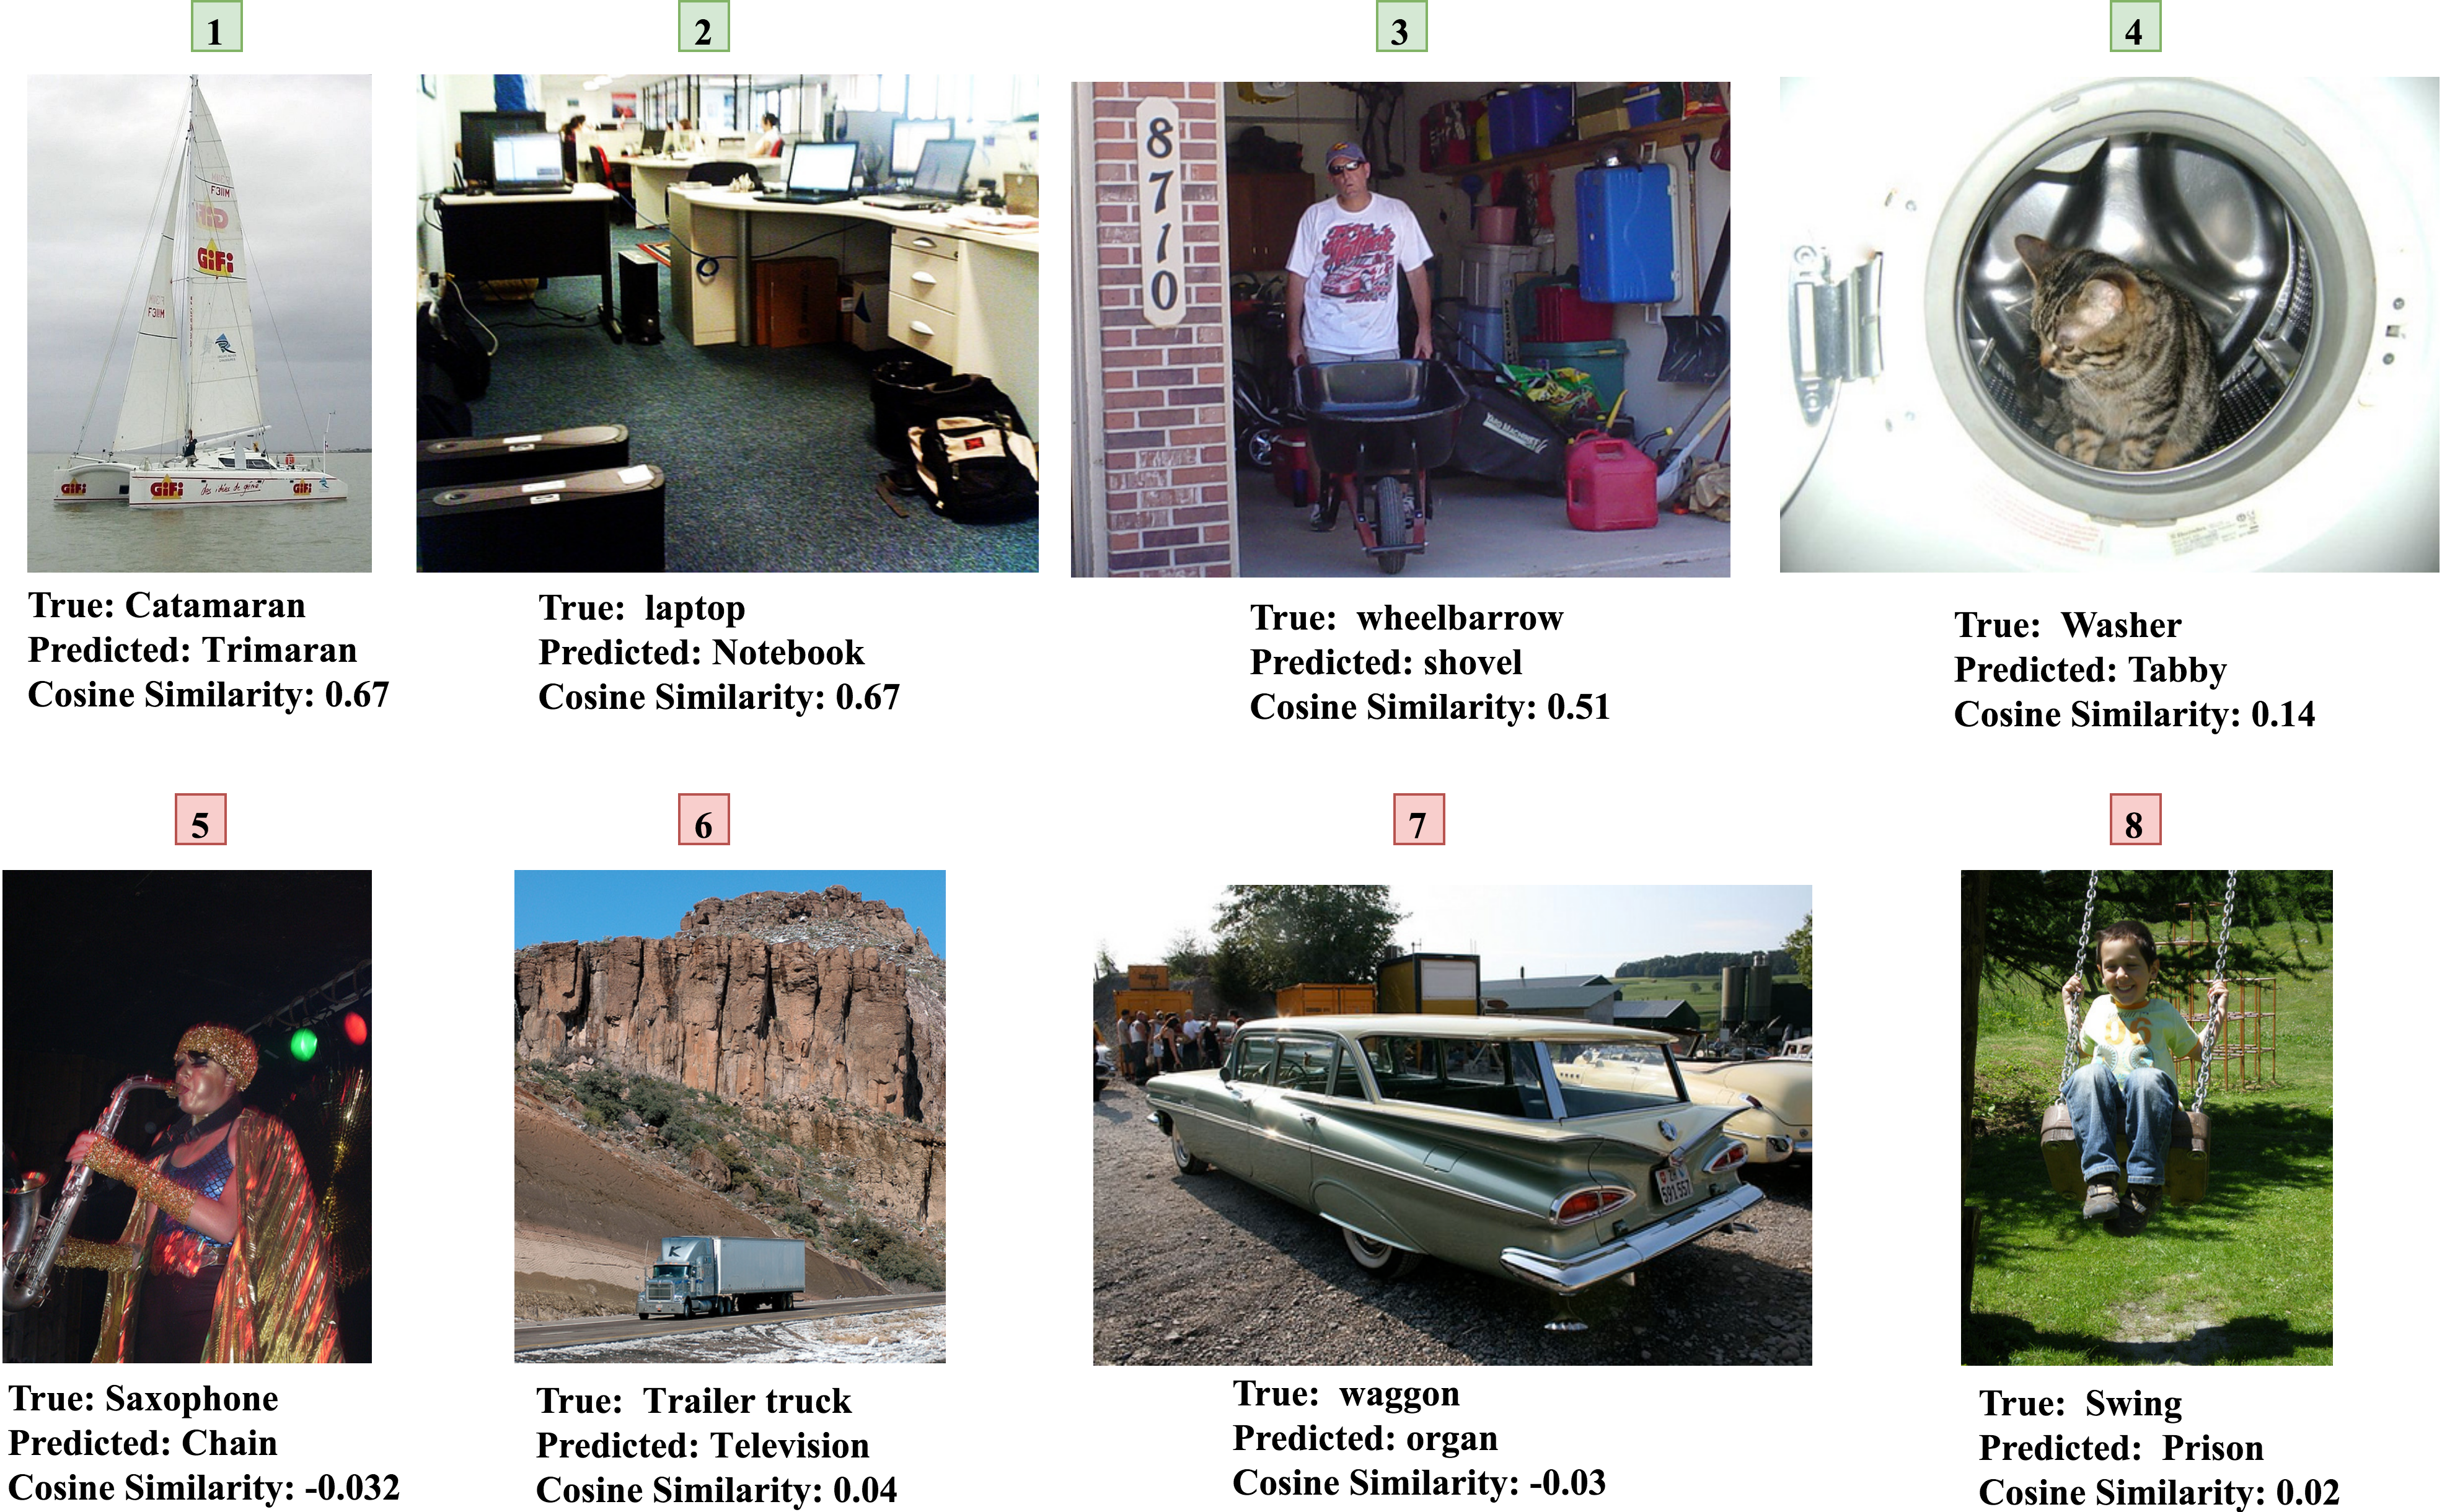
\includegraphics[width=16cm, height=12cm]{Figures/mistakes}
\caption{A qualitative analysis of the classifications mistakes of CNNs}
\label{Mistakes}
The images above were manually selected to explain the  results of 1 vs. 2 tests on VGG16, Inception-v3, and ResNet50. We consider a classification error to be serious if the cosine similarity between the true, and predicted class is small in word-vector space. Images (1-4) are considered to be small mistakes due to high cosine similarity between true, and predicted class, and is sampled from mistakes made by Inception-v3 and ResNet50. Images (5-8) are considered to be be more serious, egregious mistakes, and is sampled from mistakes made by VGG16. 

\end{figure}

Some examples of mistakes made by ResNet50 and Inception-v3 are shown under images 1-3. It should be noted that 1 vs. 2 tests only takes into account the top-1 accuracy which may not be a good measure for CNNs~\cite{ImageNETChallenge}. For example in image 3, CNN classified \textit{wheelbarrow} as a \textit{shovel}. However, there is a \textit{shovel} present in the image along with the \textit{wheelbarrow} and CNN does indeed predict \textit{wheelbarrow} correctly in its top-5 predictions. This could mean that semantics related to both \textit{wheelbarrow} and \textit{shovel} could be present in the CNN activations at the same time, and this could explain why 1 vs. 2 tests fails for these images. Moreover, both the concepts have a high similarity to each other making it even more difficult for the 1 vs. 2 tests to segregate between the semantics information of these two concepts. 

We use this reasoning to explain why VGG16 has statistically significant points in the 1 vs. 2 tests whereas ResNet50 and Inception-v3 makes smaller and acceptable top-1 mistakes and have no significant points. Another type of scenario typically seen in the misclassification by VGG16 is shown in image 4 (\textit{washer} vs \textit{tabby}). Here the top1 predicted, and actual class are dissimilar but both the concepts are present in the image and also predicted by CNN in its top-5 predictions. This could mean that semantics related to both \textit{washer} and \textit{tabby} could be present in the CNN activations at the same time but since these two concepts are dissimilar in word vector space, the 1 vs. 2 could still identify semantics of \textit{washer} from \textit{tabby}. This might explain why the fully connected layers of VGG16 is still statistically significant for 1 vs. 2 tests.

\section{Summary}


 This chapter focused on our methodology used to study the CNNs using Distributional semantic models \textit{contribution B}. The preliminary section of the chapter discussed various CNN models and DS models that were included in our experiments. The 2 vs. 2 tests designed to study the semantic representation through the various layer of the networks were also elaborated. The 1 vs. 2 tests was designed to investigate misclassifications in CNN. The results and discussion section elaborated our findings and observations. Our results indicate that CNNs do indeed learn semantics. There is an upward trend in the growth of semantic information from the initial layer to the final layer of all the three CNNs that we have studied in this thesis. In case of misclassifications, the results from the 1 vs. 2 tests indicate that the semantics for the true class is present in some layers of VGG16.
